\documentclass{beamer}

\usepackage{tikz}
\usepackage{pdfpages}
\usetikzlibrary{shapes,snakes}

\newcommand{\smtc}[1]{\texttt{#1}}
\newcommand{\smtcuc}[1]{\texttt{\color{blue}#1}}
\newcommand{\tdots}{$...$}

% switch off the fancy navigation symbols
\setbeamertemplate{navigation symbols}{}

\title{${}$\\[3.5em]12th International\\
Satisfiability Modulo Theories\\
Competition\\[.7em]
SMT-COMP 2017\\[3em]}

\author{Matthias Heizmann (co-organizer)\\ 
\and Giles Reger (co-organizer)\\ 
\and Tjark Weber (chair)\\
}

\institute{}

\date{}

\logo{\vspace{2.7cm}
\includegraphics[width=\textwidth]{laurels}\hspace{.8cm}}

\begin{document}

%%%%%%%%%%%%%%%%%%%%%%%%%%%%%%%%%%%%%%%%%%%%%%%%%%%%%%%%%%%%%%%%%%%%%%%%%%%%%%%%

\frame{\titlepage}
\logo{}

%%%%%%%%%%%%%%%%%%%%%%%%%%%%%%%%%%%%%%%%%%%%%%%%%%%%%%%%%%%%%%%%%%%%%%%%%%%%%%%%

\section{}% leave this empty
\subsection{}% leave this empty

%%%%%%%%%%%%%%%%%%%%%%%%%%%%%%%%%%%%%%%%%%%%%%%%%%%%%%%%%%%%%%%%%%%%%%%%%%%%%%%%

% \begin{frame}{SMT-COMP 2017 -- Main changes over last competition}
% 
% 
% \begin{itemize}
% \item benchmarks with 'unknown' status
% 
% \item logics with algebraic data-types (SMT-LIB 2.6 draft) 
% % \texttt{(declare-datatype, match) }
% 
% {\scriptsize AUFBVDTLIA, AUFDTLIA, QF\_DT, UFDT, UFDTLIA}
% 
% \item Unsat-core Track not ``experimental'' any more
% \end{itemize}
% 
% 
% \end{frame}


\begin{frame}{Outline}
\begin{itemize}
%  \item Brief introduction to competition procedure/rules
 \item Main changes over last competition
\begin{itemize}
\item Benchmarks with 'unknown' status

\item Logics with algebraic data-types
% \texttt{(declare-datatype, match) }

{\scriptsize AUFBVDTLIA, AUFDTLIA, QF\_DT, UFDT, UFDTLIA}

\item Unsat-core Track
\end{itemize}

\vfill

 \item Statistics and selected results of competition
 
\vfill

 \item Short presentation of solvers
 
 \small
 Boolector, COLIBRI, CVC4, SMTInterpol, veriT, Yices
 
 
\end{itemize}

 
\end{frame}



\begin{frame}{SMT-COMP -- Procedure}


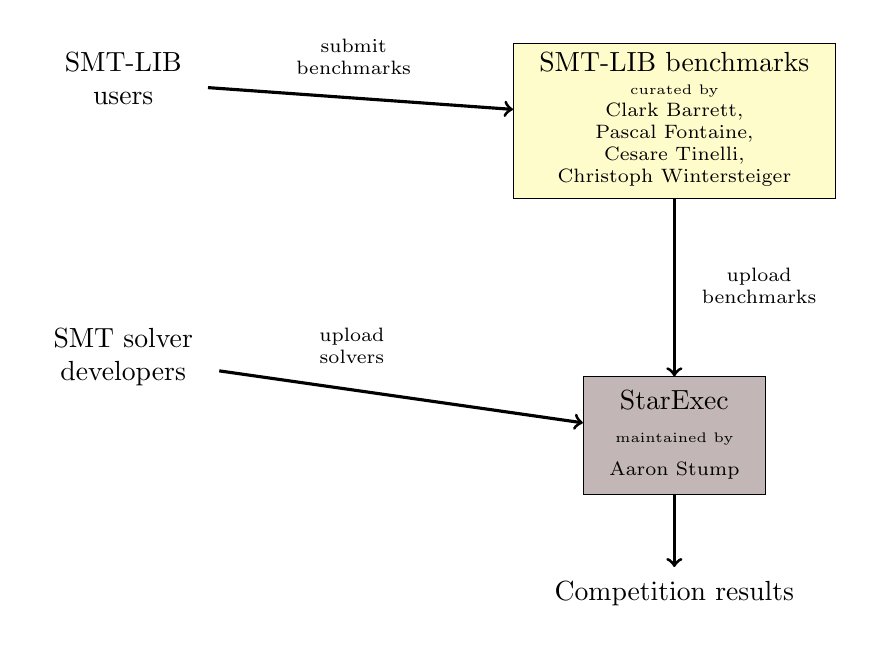
\begin{tikzpicture}
 \node (SMTusers) [] at (-7,5.5) {\begin{tabular}{c}SMT-LIB\\ users\end{tabular}};
 \node (SMTbenchmarks) [draw, rectangle, fill=yellow!20] at (0,5) {\scriptsize\begin{tabular}{c}
 \normalsize SMT-LIB benchmarks\\ \tiny curated by\\ Clark Barrett,\\ Pascal Fontaine,\\ Cesare Tinelli,\\ Christoph Wintersteiger
 \end{tabular}};
 \node (SMTsolvers) [] at (-7,2) {\begin{tabular}{c}SMT solver\\ developers\end{tabular}};
 \node (starexec) [draw, rectangle, fill=lightgray!95!red] at (0,1) {\begin{tabular}{c}StarExec\\ \tiny maintained by\\ \scriptsize Aaron Stump\end{tabular}};
 \node (results) [] at (0,-1) {\begin{tabular}{c}Competition results\end{tabular}};
 
 \draw[->,thick,line width=0.4mm] (SMTusers) to node[auto, pos=0.2] {\scriptsize \begin{tabular}{c}submit\\ benchmarks\end{tabular}} (SMTbenchmarks);
 \draw[->,thick,line width=0.4mm] (SMTsolvers) to node[auto, pos=0.2] {\scriptsize \begin{tabular}{c}upload\\ solvers\end{tabular}} (starexec);
 \draw[->,thick,line width=0.4mm] (SMTbenchmarks) to node[auto] {\scriptsize \begin{tabular}{c}upload\\ benchmarks\end{tabular}} (starexec);
  \draw[->,thick,line width=0.4mm] (starexec) to node[auto] {} (results);
      
     
%       \draw (0,-.25) -- (0,1.25);
%       \node [left] at (0,1) {\footnotesize Main track};
%       \node [left] at (0,.5) {\footnotesize Application track};
%       \node [left] at (0,0) {\footnotesize Unsat-core track};
% 
%       \draw [fill=fg] (0,.85) rectangle (2.85,1.15);
%       \node [left,white] at (2.85,1) {\footnotesize 19};
%       \draw [fill=fg!30!white] (2.85,.85) rectangle (3.15,1.15);
%       \node [right] at (3.15,1) {\tiny 2 non-competitive};
% 
%       \draw [fill=fg] (0,.35) rectangle (0.6,.65);
%       \node [left,white] at (0.6,.5) {\footnotesize 4};
%       \draw [fill=fg!30!white] (0.6,.35) rectangle (0.9,.65);
%       \node [right] at (0.9,.5) {\tiny 2 non-competitive};
% 
%       \draw [fill=fg] (0,-.15) rectangle (.3,.15);
%       \draw [fill=fg!30!white] (.3,-.15) rectangle (.6,.15);
%       \node [left,white] at (.39,0) {\footnotesize 2};
%       \node [right] at (.6,0) {\tiny 2 non-competitive};
    \end{tikzpicture}
 
\end{frame}


\begin{frame}{Solvers, Logics, and Benchmarks}
  \begin{itemize}
  \item 15 teams participated
    \smallskip
  \item Solvers:\\
    \smallskip
    \usebeamercolor{structure}
    \begin{tikzpicture}
      \draw (0,-.25) -- (0,1.25);
      \node [left] at (0,1) {\footnotesize Main track};
      \node [left] at (0,.5) {\footnotesize Application track};
      \node [left] at (0,0) {\footnotesize Unsat-core track};

      \draw [fill=fg] (0,.85) rectangle (2.85,1.15);
      \node [left,white] at (2.85,1) {\footnotesize 19};
      \draw [fill=fg!30!white] (2.85,.85) rectangle (3.15,1.15);
      \node [right] at (3.15,1) {\tiny 2 non-competitive};

      \draw [fill=fg] (0,.35) rectangle (0.6,.65);
      \node [left,white] at (0.6,.5) {\footnotesize 4};
      \draw [fill=fg!30!white] (0.6,.35) rectangle (0.9,.65);
      \node [right] at (0.9,.5) {\tiny 2 non-competitive};

      \draw [fill=fg] (0,-.15) rectangle (.3,.15);
      \draw [fill=fg!30!white] (.3,-.15) rectangle (.6,.15);
      \node [left,white] at (.39,0) {\footnotesize 2};
      \node [right] at (.6,0) {\tiny 2 non-competitive};
    \end{tikzpicture}
  \item Logics:\\
    \smallskip
    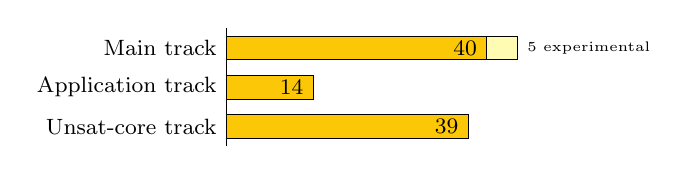
\begin{tikzpicture}
      \draw (0,-.25) -- (0,1.25);
      \node [left] at (0,1) {\footnotesize Main track};
      \node [left] at (0,.5) {\footnotesize Application track};
      \node [left] at (0,0) {\footnotesize Unsat-core track};

      \draw [fill=yellow!80!red] (0,.85) rectangle (3.30638297872,1.15);
      \node [left] at (3.30638297872,1) {\footnotesize 40};
      \draw [fill=yellow!30!white] (3.30638297872,.85) rectangle (3.7,1.15);
      \node [right] at (3.7,1) {\tiny 5 experimental};

      \draw [fill=yellow!80!red] (0,.35) rectangle (1.10212765957,.65);
      \node [left] at (1.10212765957,.5) {\footnotesize 14};

      \draw [fill=yellow!80!red] (0,-.15) rectangle (3.07021276596,.15);
      \node [left] at (3.07021276596,0) {\footnotesize 39};
    \end{tikzpicture}
  \item Benchmarks:\\
    \smallskip
    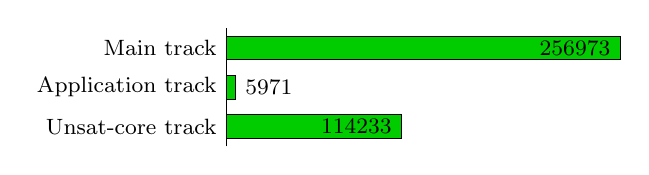
\begin{tikzpicture}
      \draw (0,-.25) -- (0,1.25);
      \node [left] at (0,1) {\footnotesize Main track};
      \node [left] at (0,.5) {\footnotesize Application track};
      \node [left] at (0,0) {\footnotesize Unsat-core track};

      \draw [fill=green!80!black] (0,.85) rectangle (5,1.15);
      \node [left] at (5,1) {\footnotesize 256973};

      \draw [fill=green!80!black] (0,.35) rectangle (0.116,.65);
      \node [right] at (0.116,.5) {\footnotesize 5971};

      \draw [fill=green!80!black] (0,-.15) rectangle (2.223,.15);
      \node [left] at (2.223,0) {\footnotesize 114233};
      
    \end{tikzpicture}
  \end{itemize}

  \vspace{-\smallskipamount}
  
%   \structure{Record number of benchmarks!}
\end{frame}


%%%%%%%%%%%%%%%%%%%%%%%%%%%%%%%%%%%%%%%%%%%%%%%%%%%%%%%%%%%%%%%%%%%%%%%%%%%%%%%%

\begin{frame}{StarExec}
Cluster of machines at the University of Iowa. 

\bigskip

  Hardware:
  \begin{itemize}
  \item Intel Xeon CPU E5-2609 @ 2.4 GHz, 10 MB cache
  \item 2 processors per node, 4 cores per processor
  \item Main memory capped at 60~GB per job pair
  \end{itemize}

  \bigskip

  Software:
  \begin{itemize}
  \item Red Hat Enterprise Linux Server release 7.2
  \item Kernel 3.10.0-514, gcc 4.8.5, glibc 2.17
  \end{itemize}

\end{frame}

%%%%%%%%%%%%%%%%%%%%%%%%%%%%%%%%%%%%%%%%%%%%%%%%%%%%%%%%%%%%%%%%%%%%%%%%%%%%%%%%


%%%%%%%%%%%%%%%%%%%%%%%%%%%%%%%%%%%%%%%%%%%%%%%%%%%%%%%%%%%%%%%%%%%%%%%%%%%%%%%%




\begin{frame}{Main Track}

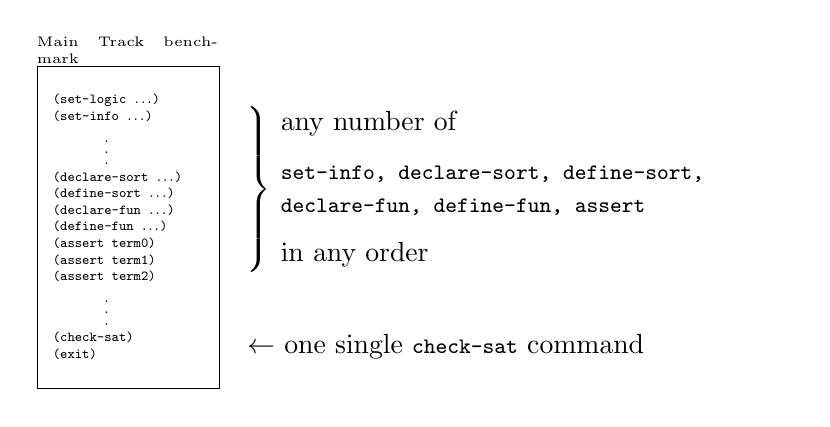
\begin{tikzpicture}
\node (maintrackscript) at (-4.1,0) {
\begin{minipage}{23mm}
\tiny

Main Track benchmark

\fbox{
\parbox{20mm}{
\strut\\
\smtc{(set-logic \tdots)}\\
\smtc{(set-info \tdots)}\\
$\phantom{mmm}\vdots$\\
\smtc{(declare-sort \tdots)}\\
\smtc{(define-sort \tdots)}\\
\smtc{(declare-fun \tdots)}\\
\smtc{(define-fun \tdots)}\\
\smtc{(assert term0)}\\
\smtc{(assert term1)}\\
\smtc{(assert term2)}\\
$\phantom{mmm}\vdots$\\
\smtc{(check-sat)}\\
\smtc{(exit)}\\
\strut
}}
\end{minipage}
};

\node[anchor=west] at (-3.1,.3) {
$\left.\begin{array}{l}\\ \\ \\ \\ \\\end{array}\right\}$
\parbox{65mm}{any number of\\[2mm] \texttt{\footnotesize set-info, declare-sort, define-sort, declare-fun, define-fun, assert}\\[2mm]
in any order}
};

\node[anchor=west] at (-2.7,-1.7) {$\leftarrow$ one single \texttt{\footnotesize check-sat} command}; 

\end{tikzpicture}
\end{frame}


\begin{frame}{Benchmarks with 'unknown' status}
Some benchmarks in SMT-LIB repository do not have a sat/unsat status.
% (around xx\% at 6th June 2017)

\vfill


{
Benchmarks with 'unknown' status in SMT-COMP
}

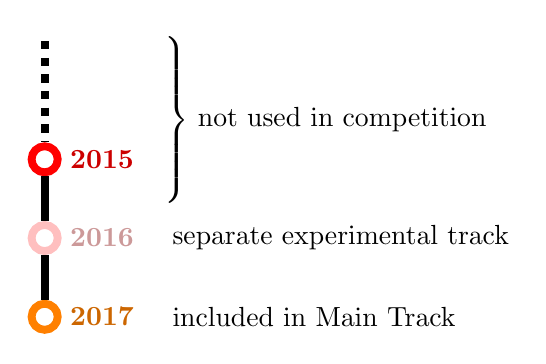
\begin{tikzpicture}
\node[circle,draw,red,line width=1mm] (2015) at (0,2) {};
\node[right of=2015, anchor=west, node distance=2mm, text=red!80!black, font=\bfseries] {2015};

\node[circle,draw,pink,line width=1mm] (2016) at (0,1) {};
\node[right of=2016, anchor=west, node distance=2mm, text=pink!80!black, font=\bfseries] {2016};

\node[circle,draw,orange,line width=1mm] (2017) at (0,0) {};
\node[right of=2017, anchor=west, node distance=2mm, text=orange!80!black, font=\bfseries] {2017};

\draw[line width=1mm, dashed] (0,3.5) to (2015);
\draw[line width=1mm] (2015) to (2016);
\draw[line width=1mm] (2016) to (2017);

\node[anchor=west] at (1,2.5) {
$\left.\begin{array}{l}\\ \\ \\ \\ \\\end{array}\right\}$ not used in competition};
\node[right of=2016, anchor=west, node distance=15mm] {separate experimental track};
\node[right of=2017, anchor=west, node distance=15mm] {included in Main Track};
\end{tikzpicture}
 
\end{frame}


\begin{frame}{New logics}
Algebraic data-types 

\begin{itemize}
 \item defined in SMT-LIB 2.6 draft
 \item ``experimental'' this year (i.e., no winner determined)
\end{itemize}


\vfill

\begin{tabular}{lrl}
& benchmarks & solvers\\ \hline
\\[-2mm]
AUFBVDTLIA & 1709 & CVC4\\[1mm]
AUFDTLIA &    728 & CVC4, vampire\\[1mm]
QF\_DT &     8000 & CVC4\\[1mm]
UFDT &       4535 & CVC4, vampire\\[1mm]
UFDTLIA &     303 & vampire, CVC4
\end{tabular}

 
 
\end{frame}




\begin{frame}{Benchmarks with 'unknown' status}
Rules
\begin{itemize}
 \item we trust the results of the solver(s)
 \item in case of disagreement we trust solvers that are sound on benchmarks with known status
 \item if there is disagreement between otherwise sound solvers, we exclude the benchmark
\end{itemize}

\vfill
\pause

Outcome
\begin{itemize}
 \item There were 29 benchmarks with unknown status 
%  (=xx\%) 
 on which solvers disagreed on the result.
 \item On one benchmark (in BV) the corresponding solvers were sound on all benchmarks with known status.
 \item On 28 benchmarks (all in QF\_FP) the presumably wrong answers were given by unsound solvers. 
\end{itemize}


\end{frame}



\begin{frame}{Competition run of Main Track}
\begin{itemize}
 \item run all job pairs with \structure{10 min timeout}
 \item made preliminary results available
 \item rerun all job pairs that timed out with \structure{20 min timeout}
 \item made final results available on Friday (21st June)
\end{itemize}

 
\end{frame}


\begin{frame}{Main Track -- Selected results -- QF\_ABV}

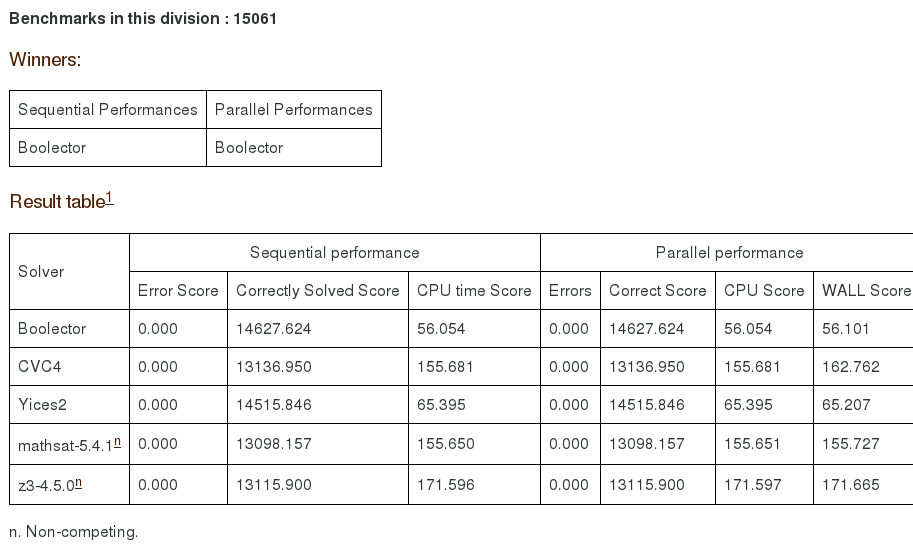
\includegraphics[width=11cm]{screenshots/Results-QF_ABV}

\texttt{\tiny http://smtcomp.sourceforge.net/2017/results-QF\_ABV.shtml}
\end{frame}



%%%%%%%%%%%%%%%%%%%%%%%%%%%%%%%%%%%%%%%%%%%%%%%%%%%%%%%%%%%%%%%%%%%%%%%%%%%%%%%%

\begin{frame}{Main Track: Competition-Wide Scoring}
  \begin{tabular}{llrr}
    Rank & Solver & Score (sequential) & Score (parallel)\\ \hline
         & \textcolor{gray}{Z3} & \textcolor{gray}{171.99} & \textcolor{gray}{171.99} \\
    1    & CVC4   & 161.38             & 161.76 \\
    2    & Yices2  & 110.63             & 110.63 \\
    3    & SMTInterpol  & 65.96              & 66.00 \\
  \end{tabular}  
\end{frame}

%%%%%%%%%%%%%%%%%%%%%%%%%%%%%%%%%%%%%%%%%%%%%%%%%%%%%%%%%%%%%%%%%%%%%%%%%%%%%%%%




\begin{frame}{Application Track}

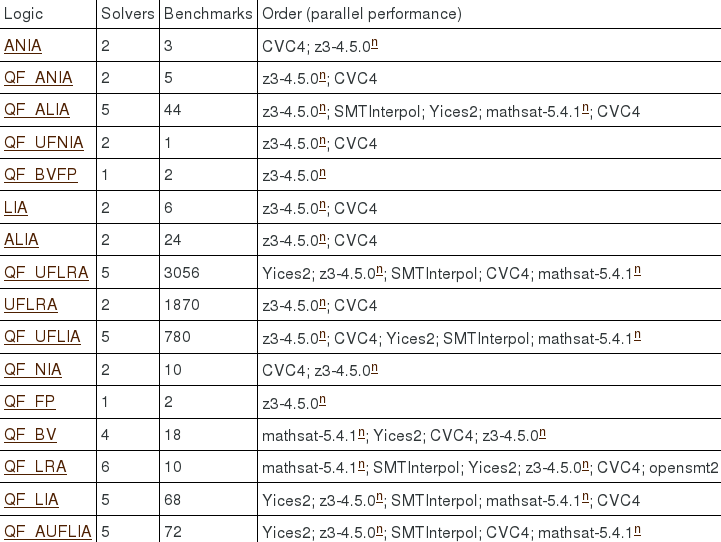
\includegraphics[width=11cm]{screenshots/Results-ApplicationTrack}

% \texttt{\tiny http://smtcomp.sourceforge.net/2017/results-QF\_ABV.shtml}
\end{frame}


%%%%%%%%%%%%%%%%%%%%%%%%%%%%%%%%%%%%%%%%%%%%%%%%%%%%%%%%%%%%%%%%%%%%%%%%%%%%%%%%



\begin{frame}{Unsat-core Track}

Motivation
\begin{itemize}
\item Important application of SMT-LIB
\item One step towards verifiable proofs
\end{itemize}

\bigskip

History
% \begin{itemize}
%  \item First introduced in 2012, discontinued in 2013
%  \item reinstated in 2016 as experimental track
%  \item ``Regular'' track in 2017
% \end{itemize}

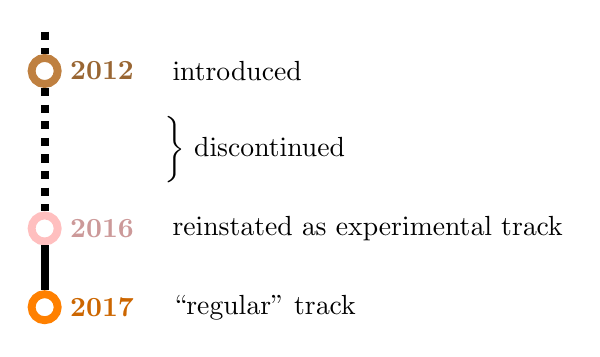
\begin{tikzpicture}
\node[circle,draw,brown,line width=1mm] (2012) at (0,3) {};
\node[right of=2012, anchor=west, node distance=2mm, text=brown!80!black, font=\bfseries] {2012};

\node[circle,draw,pink,line width=1mm] (2016) at (0,1) {};
\node[right of=2016, anchor=west, node distance=2mm, text=pink!80!black, font=\bfseries] {2016};

\node[circle,draw,orange,line width=1mm] (2017) at (0,0) {};
\node[right of=2017, anchor=west, node distance=2mm, text=orange!80!black, font=\bfseries] {2017};


\draw[line width=1mm, dashed] (0,3.5) to (2012);
\draw[line width=1mm, dashed] (2012) to (2016);
\draw[line width=1mm] (2016) to (2017);

\node[right of=2012, anchor=west, node distance=15mm] {introduced};
\node[anchor=west] at (1,2) {
$\left.\begin{array}{l}\\ \\\end{array}\right\}$ discontinued};
\node[right of=2016, anchor=west, node distance=15mm] {reinstated as experimental track};
\node[right of=2017, anchor=west, node distance=15mm] {``regular'' track};
\end{tikzpicture}

 
\end{frame}



\begin{frame}{Unsat-core Track}
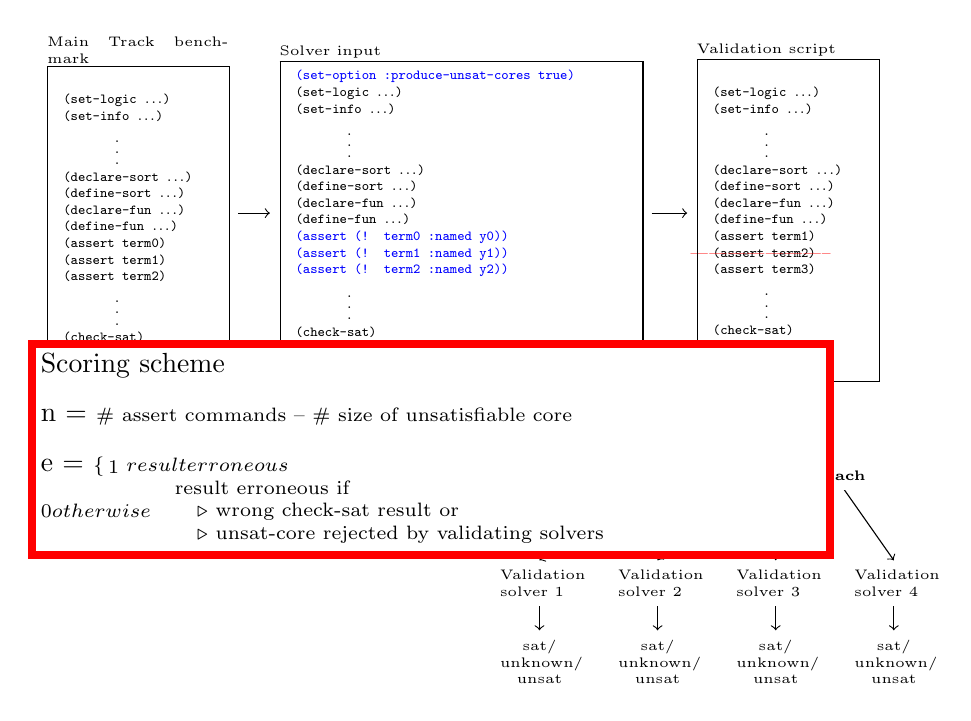
\begin{tikzpicture}
\node (maintrackscript) at (-4.1,0) {
\begin{minipage}{23mm}
\tiny

Main Track benchmark

\fbox{
\parbox{20mm}{
\strut\\
\smtc{(set-logic \tdots)}\\
\smtc{(set-info \tdots)}\\
$\phantom{mmm}\vdots$\\
\smtc{(declare-sort \tdots)}\\
\smtc{(define-sort \tdots)}\\
\smtc{(declare-fun \tdots)}\\
\smtc{(define-fun \tdots)}\\
\smtc{(assert term0)}\\
\smtc{(assert term1)}\\
\smtc{(assert term2)}\\
$\phantom{mmm}\vdots$\\
\smtc{(check-sat)}\\
\smtc{(exit)}\\
\strut
}}
\end{minipage}
};



\node (solverinput) at (0,0) {
\begin{minipage}{46mm}
\tiny

Solver input

\fbox{
\parbox{43mm}{
\smtcuc{(set-option  :produce-unsat-cores true)}\\
\smtc{(set-logic \tdots)}\\
\smtc{(set-info \tdots)}\\
$\phantom{mmm}\vdots$\\
\smtc{(declare-sort \tdots)}\\
\smtc{(define-sort \tdots)}\\
\smtc{(declare-fun \tdots)}\\
\smtc{(define-fun \tdots)}\\
\smtcuc{(assert (! term0 :named y0))}\\
\smtcuc{(assert (! term1 :named y1))}\\
\smtcuc{(assert (! term2 :named y2))}\\
$\phantom{mmm}\vdots$\\
\smtc{(check-sat)}\\
\smtcuc{(get-unsat-core)}\\
\smtc{(exit)}
}}
\end{minipage}
};
\draw[->] (maintrackscript) to (solverinput);

\pause


\node (solveroutput) at (0,-3.2) {
\begin{minipage}{16mm}
\tiny

Solver output

\fbox{
\parbox{12mm}{
\smtc{unsat}\\
\smtc{(y0 y2)}
}}
\end{minipage}
};
\draw[->, bend right, out=-90] (solverinput.south west) to node[left]{\tiny\textbf{timeout: 40min}} (solveroutput.west);

\pause

\node (validationscript) at (4.0,0) {
\begin{minipage}{20mm}
\tiny

Validation script

\fbox{
\parbox{20mm}{
\strut\\
\smtc{(set-logic \tdots)}\\
\smtc{(set-info \tdots)}\\
$\phantom{mmm}\vdots$\\
\smtc{(declare-sort \tdots)}\\
\smtc{(define-sort \tdots)}\\
\smtc{(declare-fun \tdots)}\\
\smtc{(define-fun \tdots)}\\
\smtc{(assert term1)}\\
\smtc{(assert term2)}{\color{red}\hspace{-16mm}-----------------------}\\
\smtc{(assert term3)}\\
$\phantom{mmm}\vdots$\\
\smtc{(check-sat)}\\
\smtc{(exit)}\\
\strut
}}
\end{minipage}
};

\draw[->] (solverinput) to (validationscript);

\draw[->, bend right, out=-20] (solveroutput.east) to (validationscript.south west);



\pause

\node (valoutput1) at (1,-4.7) {
\begin{minipage}{10mm}
\tiny

Validation\\ solver 1

\end{minipage}
};

\node (valoutput2) at (2.5,-4.7) {
\begin{minipage}{10mm}
\tiny

Validation\\ solver 2

\end{minipage}
};

\node (valoutput3) at (4,-4.7) {
\begin{minipage}{10mm}
\tiny

Validation\\ solver 3

\end{minipage}
};

\node (valoutput4) at (5.5,-4.7) {
\begin{minipage}{10mm}
\tiny

Validation\\ solver 4
\end{minipage}
};



\node[below of=valoutput1] (valoutput1res) {
\begin{minipage}{10mm}
\tiny\centering
sat/\\
unknown/\\
unsat
\end{minipage}
};

\node[below of=valoutput2] (valoutput2res) {
\begin{minipage}{10mm}
\tiny\centering
sat/\\
unknown/\\
unsat
\end{minipage}
};

\node[below of=valoutput3] (valoutput3res) {
\begin{minipage}{10mm}
\tiny\centering
sat/\\
unknown/\\
unsat
\end{minipage}
};

\node[below of=valoutput4] (valoutput4res) {
\begin{minipage}{10mm}
\tiny\centering
sat/\\
unknown/\\
unsat
\end{minipage}
};




\draw[->] (validationscript.south) to (valoutput1.north);
\draw[->] (validationscript.south) to (valoutput2.north);
\draw[->] (validationscript.south) to (valoutput4.north);
\draw[->] (validationscript.south) to node[fill=white]{\tiny\textbf{timeout: 5min each}} (valoutput3.north);



\draw[->] (valoutput1) to (valoutput1res);
\draw[->] (valoutput2) to (valoutput2res);
\draw[->] (valoutput3) to (valoutput3res);
\draw[->] (valoutput4) to (valoutput4res);

\pause

\node[fill=white,draw=red, line width=1mm, anchor=west] (scoring) at (-5.5,-3) {
\begin{minipage}{99mm}
Scoring scheme


\medskip


n = {\scriptsize  \# assert commands -- \# size of unsatisfiable core}

\medskip

e = {\scriptsize $\begin{cases}
1 \text{ result erroneous}\\
0 \text{ otherwise}
   \end{cases}
$
\begin{tabular}{l}
result erroneous if\\
$\quad\triangleright$ wrong check-sat result or\\
$\quad\triangleright$ unsat-core rejected by validating solvers
\end{tabular}
}
\end{minipage}
};




\end{tikzpicture}
 
\end{frame}


% \begin{frame}{Unsat-core Track -- Statistics}
% 
% \begin{tabular}{rl}
%  245483 & job pairs\\
%  226501 & correct check-sat responses\\
%      29 & incorrect check-sat responses\\
%  226471 & get-unsat-core responses\\
%  226463 & times the unsatisfiable core was validated\\
%       8 & times the unsatisfiable core was not correct\\
%       8 & times the unsatisfiable core was invalidated by the same solver\\
%      19 & times there was no consensus among the validating solvers\\
%   27525 & times no independent validating solver approved the correctness of the unsatisfiable core
% \end{tabular}
% 
% \end{frame}



\begin{frame}{Unsat-core Track -- Statistics}

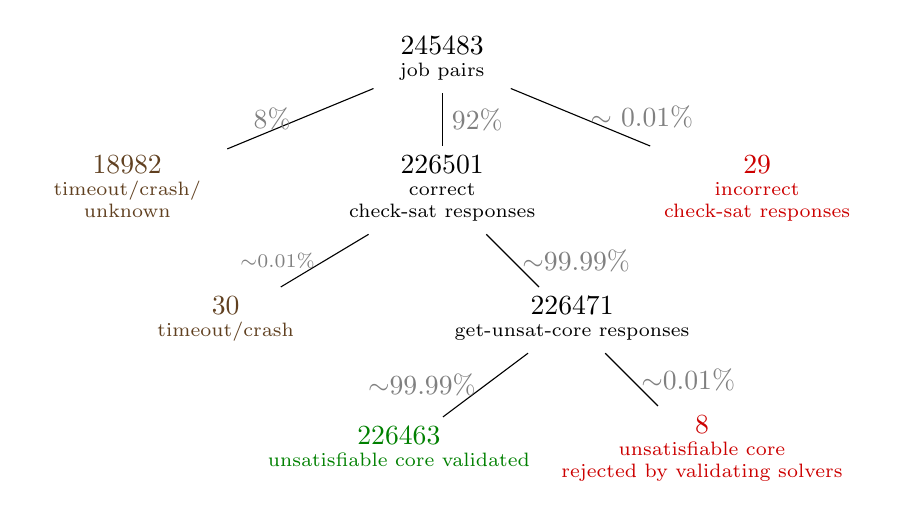
\begin{tikzpicture}[scale=1.1]
\node[] (jobpairs) at (0,0) { 
\scriptsize 
\begin{tabular}{c}\normalsize 245483\\ job pairs\end{tabular} 
}; 

\node[] (unsat) at (-0.0, -1.5) { 
\scriptsize 
\begin{tabular}{c}\normalsize 226501\\ correct\\ check-sat responses\end{tabular} 
}; 
\draw (jobpairs) to (unsat);

\node[left of=unsat, node distance=40mm, text=brown!50!black] (unknown) { 
\scriptsize 
\begin{tabular}{c}\normalsize 18982\\ timeout/crash/\\unknown\end{tabular} 
}; 

\node[right of=unsat, node distance=40mm, text=red!80!black] (sat) {
\scriptsize 
\begin{tabular}{c}\normalsize 29\\ incorrect\\ check-sat responses\end{tabular} 
};
\draw[auto] (jobpairs) to node[text=gray] {92\%} (unsat);
\draw[left] (jobpairs) to node[text=gray] {8\%} (unknown);
\draw[right] (jobpairs) to node[text=gray] {$\sim$ 0.01\%} (sat);

\node[text=brown!50!black] (nouc) at (-2.5,-3) { 
\scriptsize 
\begin{tabular}{c}\normalsize 30\\ timeout/crash\end{tabular} 
}; 

\node[] (uc) at (1.5,-3) { 
\scriptsize 
\begin{tabular}{c}\normalsize 226471\\ get-unsat-core responses\end{tabular} 
}; 

\draw[left] (unsat) to node[text=gray] {\scriptsize $\sim$0.01\%} (nouc);
\draw[right] (unsat) to node[text=gray] {$\sim$99.99\%} (uc);


\node[text=red!80!black] (rejected) at (3,-4.5) { 
\scriptsize 
\begin{tabular}{c}\normalsize 8\\ unsatisfiable core\\ rejected by validating solvers\end{tabular} 
}; 

\node[text=green!50!black] (validated) at (-0.5,-4.5) { 
\scriptsize 
\begin{tabular}{c}\normalsize 226463\\ unsatisfiable core validated\end{tabular} 
}; 

\draw[right] (uc) to node[text=gray] {$\sim$0.01\%} (rejected);
\draw[left] (uc) to node[text=gray] {$\sim$99.99\%} (validated);

\end{tikzpicture}


\pause

\begin{itemize}
\item 19 times there was no consensus among the validating solvers ($\rightsquigarrow$ majority decision)
\item 27525 ($\sim$12\%) times no independent validating solver approved the correctness of the unsatisfiable core
\end{itemize}



% \scriptsize
% \begin{tabular}{rl}
% %  226463 & times the unsatisfiable core was validated\\
% %       8 & times the unsatisfiable core was not correct\\
% %       8 & times the unsatisfiable core was invalidated by the same solver\\
%      19 & times there was no consensus among the validating solvers\\
%   27525 & times no independent validating solver approved the correctness of the unsatisfiable core
% \end{tabular}




% \begin{tabular}{rl}
%  245483 & job pairs\\
%  226501 & correct check-sat responses\\
%      29 & incorrect check-sat responses\\
%  226471 & get-unsat-core responses\\
%  226463 & times the unsatisfiable core was validated\\
%       8 & times the unsatisfiable core was not correct\\
%       8 & times the unsatisfiable core was invalidated by the same solver\\
%      19 & times there was no consensus among the validating solvers\\
%   27525 & times no independent validating solver approved the correctness of the unsatisfiable core
% \end{tabular}

\end{frame}


 
% Divisions where sometimes no independent validating solver approved 
% correctness of the unsatisfiable core
% [ALIA, AUFLIRA, AUFNIRA, BV, LRA, QF_ABV, NRA, QF_ALIA, QF_AUFLIA, QF_BV, 
% QF_AX, QF_BVFP, QF_FP, QF_IDL, QF_LIA, QF_LIRA, QF_LRA, QF_NIA, QF_NRA, QF_UF, 
% QF_RDL, QF_UFIDL, QF_UFBV, UF, UFBV, UFLIA, UFNIA]















\logo{}

%%%%%%%%%%%%%%%%%%%%%%%%%%%%%%%%%%%%%%%%%%%%%%%%%%%%%%%%%%%%%%%%%%%%%%%%%%%%%%%%

\begin{frame}{}
(Very) short presentations of

  \begin{center}
    \vfill
    
      {\huge \structure{Solvers}}
      
    \vfill
  \end{center}
      that sent us slides.

    \vfill
\begin{center}
Boolector, COLIBRI, CVC4, SMTInterpol, veriT, Yices
\end{center}

\end{frame}

{
  \setbeamercolor{background canvas}{bg=}
  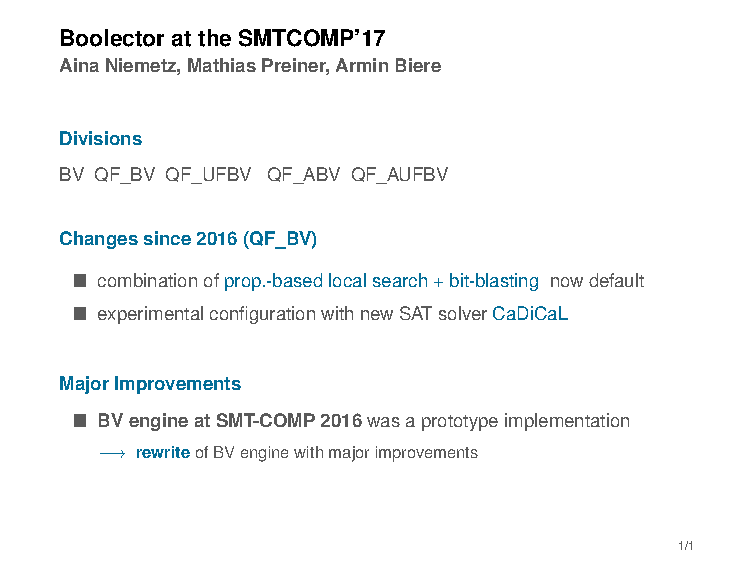
\includepdf[pages={1-}]{solvers/Boolector.pdf}
  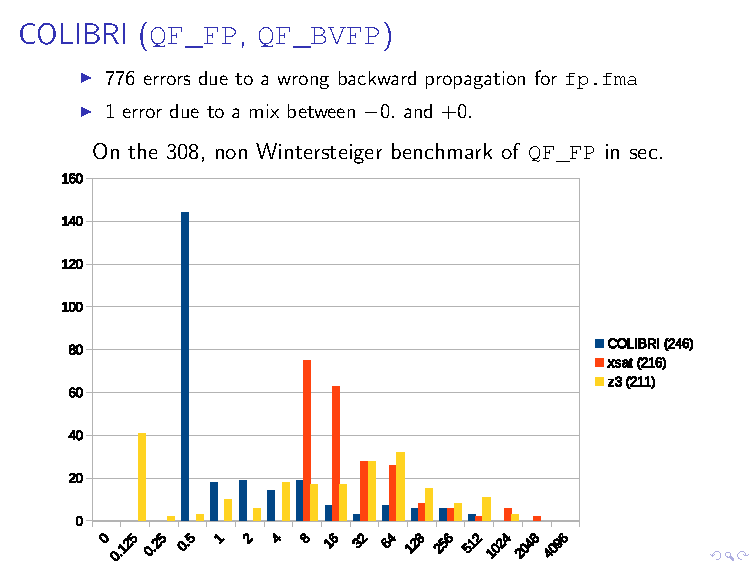
\includepdf[pages={1-}]{solvers/COLIBRI.pdf}
  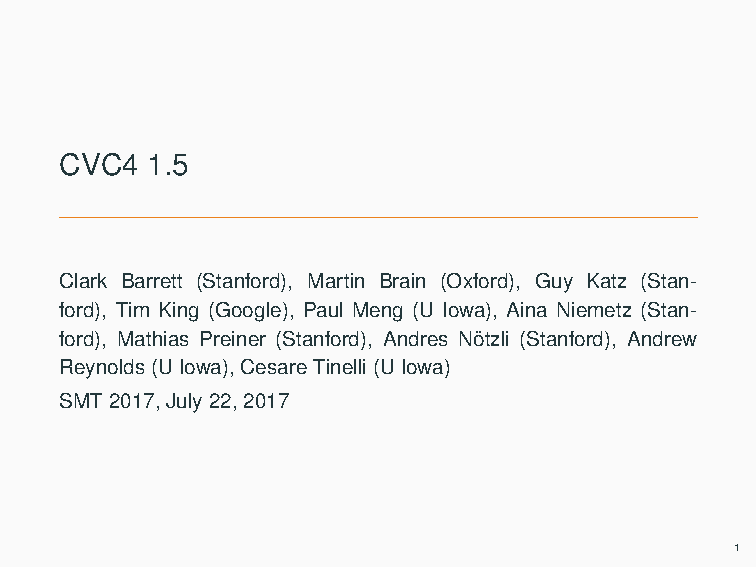
\includepdf[pages={1-}]{solvers/CVC4.pdf}
  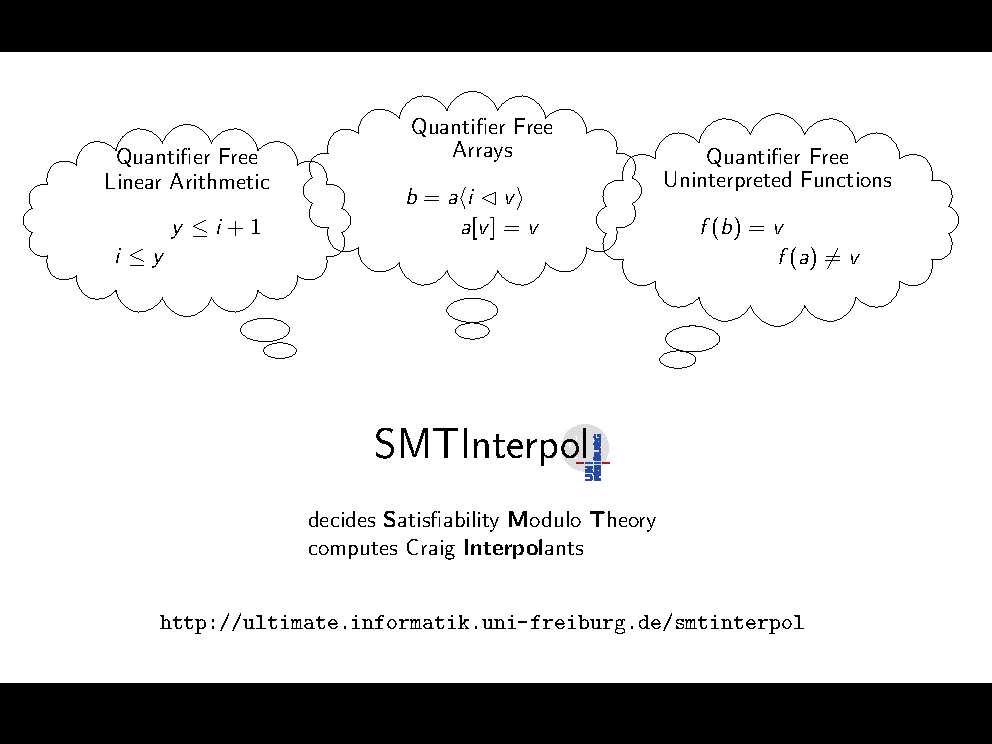
\includepdf[pages={1-}]{solvers/SMTInterpol.pdf}
  
\includepdf[pages={1-}]{solvers/veriT.pdf}
  
\includepdf[pages={1-}]{solvers/Yices.pdf}
}

% %%%%%%%%%%%%%%%%%%%%%%%%%%%%%%%%%%%%%%%%%%%%%%%%%%%%%%%%%%%%%%%%%%%%%%%%%%%%%%%%
% 
% \begin{frame}{}
%   \begin{center}
%     \vfill
%       {\huge \structure{Selected Results}}
%     \vfill
%   \end{center}
% \end{frame}
% 
% %%%%%%%%%%%%%%%%%%%%%%%%%%%%%%%%%%%%%%%%%%%%%%%%%%%%%%%%%%%%%%%%%%%%%%%%%%%%%%%%
% 
% \begin{frame}{Results: QF\_BV (Main Track)}
%   \begin{tabular}{lrrr}
% Solver          & Error Score & Solved Score (Parallel) & Unsolved \\ \hline
% {\bf Boolector (pre)} & {\bf 0.000} & {\bf 24473.995} & {\bf 149} \\
% Boolector 	& 0.000	& 24468.395 & 150 \\
% Minkeyrink 	& 0.000	& 24434.194 & 193 \\
% smt-cms-mt 	& 0.000	& 24244.599 & 216 \\
% smt-cms-st 	& 0.000	& 24165.007 & 214 \\
% CVC4 	        & 0.000	& 23820.707 & 231 \\
% \textcolor{gray}{Z3} & \textcolor{gray}{0.000} & \textcolor{gray}{23732.215} & \textcolor{gray}{304} \\
% smt-cms-exp 	& 0.000	& 23640.669 & 270 \\
% ABC\_glucose 	& 0.000	& 23078.931 & 477 \\
% Yices2 	        & 0.000	& 22687.777 & 638 \\
% \textcolor{gray}{MathSat5} & \textcolor{gray}{0.000} & \textcolor{gray}{22496.779} & \textcolor{gray}{544} \\
% MapleSTP-mt 	& 0.000	& 22487.264 & 395 \\
% MapleSTP 	& 0.000	& 21764.885 & 450 \\
% smt-minisat-st 	& 0.000	& 20582.614 & 1058 \\
% ABC\_default 	& 0.000	& 18528.788 & 1354 \\
% Q3B 	        & 719.723 & 10397.757 & 4430
%   \end{tabular}  
% \end{frame}
% 
% %%%%%%%%%%%%%%%%%%%%%%%%%%%%%%%%%%%%%%%%%%%%%%%%%%%%%%%%%%%%%%%%%%%%%%%%%%%%%%%%
% 
% \begin{frame}{Results: Competition-Wide Scoring (Main Track)}
%   \begin{tabular}{llrr}
%     Rank & Solver & Score (sequential) & Score (parallel)\\ \hline
%          & \textcolor{gray}{Z3} & \textcolor{gray}{185.09} & \textcolor{gray}{185.09} \\
%     1    & CVC4   & 180.95             & 181.19 \\
%     2    & Yices  & 119.29             & 119.29 \\
%     3    & veriT  & 75.11              & 75.11 \\
%     \\
%     \\
%     \multicolumn{3}{l}{Best newcomer:}\\
%     \\
%     5    & Vampire\_parallel & 65.36 & 65.62	
%   \end{tabular}  
% \end{frame}
% 
% %%%%%%%%%%%%%%%%%%%%%%%%%%%%%%%%%%%%%%%%%%%%%%%%%%%%%%%%%%%%%%%%%%%%%%%%%%%%%%%%
% 
% \begin{frame}{Results: Application Track (Summary)}
%   \begin{tabular}{ll}
%     Logic       & Order \\ \hline
%     ANIA	& \textcolor{gray}{Z3; CVC4} \\
%     QF\_ANIA	& \textcolor{gray}{Z3; CVC4} \\
%     QF\_ALIA	& \textcolor{gray}{Z3;} SMTInterpol; Yices2; \textcolor{gray}{MathSat5; CVC4} \\
%     QF\_UFNIA	& \textcolor{gray}{Z3; CVC4} \\
%     LIA         & \textcolor{gray}{Z3; CVC4} \\
%     ALIA	& \textcolor{gray}{Z3; CVC4} \\
%     QF\_UFLRA	& \textcolor{gray}{Z3}; Yices2; SMTInterpol; \textcolor{gray}{CVC4; MathSat5} \\
%     UFLRA	& \textcolor{gray}{Z3; CVC4} \\
%     QF\_UFLIA	& \textcolor{gray}{Z3; CVC4;} Yices2; SMTInterpol; \textcolor{gray}{MathSat5} \\
%     QF\_NIA	& \textcolor{gray}{CVC4; Z3} \\
%     QF\_BV	& \textcolor{gray}{MathSat5;} Yices2; smt-cms-st; smt-cms-mt; \\
%     & \quad smt-cms-exp; \textcolor{gray}{CVC4;} MapleSTP; MapleSTP-mt; \\
%     & \quad smt-minisat-st; \textcolor{gray}{Z3} \\
%     QF\_LRA	& \textcolor{gray}{MathSat5;} SMTInterpol; \textcolor{gray}{Z3}; Yices2; \textcolor{gray}{CVC4} \\
%     QF\_LIA	& Yices2; \textcolor{gray}{Z3}; SMTInterpol; \textcolor{gray}{MathSat5; CVC4} \\
%     QF\_AUFLIA	& Yices2; \textcolor{gray}{Z3}; SMTInterpol; \textcolor{gray}{MathSat5; CVC4}
%   \end{tabular}
% \end{frame}
% 
% %%%%%%%%%%%%%%%%%%%%%%%%%%%%%%%%%%%%%%%%%%%%%%%%%%%%%%%%%%%%%%%%%%%%%%%%%%%%%%%%
% 
% \begin{frame}{Selected Results: Unsat-Core Track}
%   \begin{tabular}{lrr}
%     Solver & Errors & Reductions \\ \hline
%     SMTInterpol                & 0                       & 1166535 \\
%     \textcolor{gray}{toysmt}   & \textcolor{gray}{0}     & \textcolor{gray}{35886} \\
%     \textcolor{gray}{veriT}    & \textcolor{gray}{26}    & \textcolor{gray}{68811} \\
%     \textcolor{gray}{MathSat5} & \textcolor{gray}{190}   & \textcolor{gray}{1527159} \\
%     \textcolor{gray}{Z3}       & \textcolor{gray}{17079} & \textcolor{gray}{4597883}
%   \end{tabular}
%   \bigskip
% 
% \end{frame}
% 
% %%%%%%%%%%%%%%%%%%%%%%%%%%%%%%%%%%%%%%%%%%%%%%%%%%%%%%%%%%%%%%%%%%%%%%%%%%%%%%%%


\begin{frame}{
% Further Thoughts
}
%   We need better tool support:
%   \begin{itemize}
%    \item Support for algebraic data types in benchmark scrambler
%   \end{itemize}
% 
%   
% \vfill
% 
% Reduce gap between competition and SMT-LIB applications.
% 
% \begin{itemize}
%  \item Nested arrays
%  \item Integer division and modulo
%  \item Model production
%  \item Interpolation
% \end{itemize}
% 
% \vfill

  Teams:
  \begin{itemize}
  \item \structure{Congratulations on your accomplishments!}
  \item \structure{Thanks for your participation!}
  \end{itemize}
\end{frame}

%%%%%%%%%%%%%%%%%%%%%%%%%%%%%%%%%%%%%%%%%%%%%%%%%%%%%%%%%%%%%%%%%%%%%%%%%%%%%%%%

\end{document}

%%%%%%%%%%%%%%%%%%%%%%%%%%%%%%%%%%%%%%%%%%%%%%%%%%%%%%%%%%%%%%%%%%%%%%%%%%%%%%%%

% Local Variables:
% ispell-local-dictionary: "american"
% mode: LaTeX
% mode: flyspell
% LocalWords: curation logics satisfiability Tjark
% End:
